\documentclass{sn-article}
\raggedbottom
\usepackage{amssymb}
\usepackage{graphicx}
\usepackage{booktabs}
\usepackage{graphicx}
\usepackage{amsmath, amssymb}
\usepackage[numbers]{natbib}
\usepackage{caption}
\usepackage{subcaption} % if you use subfigures
\usepackage{hyperref}
\usepackage{booktabs}
\usepackage{float}
\usepackage[table]{xcolor}
\usepackage[colorlinks=true,allcolors=blue]{hyperref}
\usepackage{amsmath,amsfonts}
\usepackage{textcomp}
\usepackage{graphicx}
\hyphenation{op-tical net-works semi-conduc-tor IEEE-Xplore}
% updated with editorial comments 8/9/2021

\section
\subsubsection{\@startsection{subsubsection}{3}{\z@}%
  {0.75\baselineskip} % space before
  {0.25\baselineskip} % space after
  {\normalfont\normalsize}}
\subsubsection

\begin{document}

\title{Temporal Patterns and Pixel Precision: Satellite-Based Crop Classification Using Deep Learning and Machine Learning}

\author{Sairam Venkatachalam \and Disha Kacha \and Devarsh Sheth \and Michael Mann \and Amir Jafari}

\institute{
Sairam Venkatachalam \and Disha Kacha \and Devarsh Sheth \\
Department of Geography \& Environment and the Data Science Program, \\
The George Washington University, Washington DC, USA \\
\email{sairam.venkatachalam@gwu.edu, disha.kacha@gwu.edu, devarshapurva.sheth@gwu.edu}
\and
Michael Mann \and Amir Jafari \\
Department of Geography \& Environment, \\
The George Washington University, Washington DC, USA \\
\email{mmann1123@email.gwu.edu, ajafari@email.gwu.edu}
}

\title{Temporal Patterns and Pixel Precision: Satellite-Based Crop Classification Using Deep Learning and Machine Learning}

\maketitle

\begin{abstract}
Accurate crop classification using satellite imagery is crucial for agricultural monitoring, yield forecasting, and sustainable resource management. However, existing methods face persistent challenges due to the spectral similarity between crop types, the incomplete exploitation of temporal dynamics, and the reliance on hand-crafted or generated features that limit generalizability. Traditional machine learning models often fail to fully leverage the rich spatiotemporal information inherent in multi-temporal optical Earth observation datasets such as Sentinel-2. To address these gaps, we developed and compared advanced deep learning models, including a CNN-BiLSTM hybrid, a TabTransformer ensemble, and a 3D CNN ensemble, that directly model raw pixel sequences across spectral bands and vegetation indices without depending on manually engineered features. We benchmarked these against classical machine learning approaches (e.g., XGBoost, Random Forest) enhanced with automated feature extraction via \texttt{xr\_fresh}. Our results show that while a voting-based machine learning classifier outperformed some deep learning models at the pixel level, the CNN-BiLSTM ensemble achieved the highest field-level performance, with a Cohen’s Kappa of 0.77 and F1 score of 0.84, surpassing traditional methods by over 0.1 in key metrics. Notably, this was accomplished without hand-crafted features, highlighting the model’s ability to learn robust representations from raw temporal data. By integrating sequence-based modeling, ensemble strategies, and data balancing techniques, our research advances the current state-of-the-art in crop classification and addresses key limitations in prior work. These findings offer meaningful improvements to remote sensing-based agricultural monitoring systems and establish a foundation for more scalable and generalizable crop classification pipelines.$$
\end{abstract}

\keywords{Crop classification, Satellite imagery, Deep learning, Machine learning, Remote sensing}


\maketitle
%%%%%%%%%%%%%%%%%%%%%%%%%%%%%%%%%%%%%%%%%%%%%%%%%%%%%%%%%%%%%%%%%%%%%%%%%%%%%%
%% Main text
%%%%%%%%%%%%%%%%%%%%%%%%%%%%%%%%%%%%%%%%%%%%%%%%%%%%%%%%%%%%%%%%%%%%%%%%%%%%%%

\section{Introduction}

Accurate and timely crop classification is foundational to precision agriculture, enabling yield forecasting, resource optimization, food security assessment, and climate-resilient decision-making \cite{mdpi2023, sciencedirect2023, ieee2017}. The widespread availability of high-resolution Earth observation data, especially from the Sentinel-2 satellite constellation, has transformed the landscape of agricultural monitoring. With 13 spectral bands, spatial resolutions ranging from 10 to 60 meters, and a revisit frequency of approximately five days, Sentinel-2 offers dense multi-temporal imagery rich in spatial and spectral information \cite{arxiv2024}.

Despite these advancements, reliable crop classification remains a complex task. Spectral similarities between crops, temporal variability in planting and phenological cycles, and atmospheric disturbances such as cloud cover hinder classification accuracy.Traditional machine learning methods often rely heavily on manually engineered features, such as vegetation indices or statistical summaries, which may capture limited temporal dynamics and can lack generalizability across different agricultural contexts. While we include indices like the Enhanced Vegetation Index (EVI) as part of our input data, they serve as complementary signals rather than sole inputs. Our deep learning models ingest both raw spectral bands and derived indices, enabling them to learn rich, multiscale spatiotemporal patterns directly from the data, beyond what handcrafted features can provide in isolation. This hybrid approach bridges domain knowledge with end-to-end representation learning for improved accuracy and scalability. 

This study addresses a critical gap in the literature: the lack of robust, scalable crop classification pipelines that fully leverage the temporal depth of Sentinel-2 optical imagery without dependence on synthetic-aperture radar (SAR) or manual feature engineering. While SAR is widely recognized for its all-weather imaging capabilities and complementary spectral characteristics, we intentionally focus solely on optical data to assess the standalone potential of multi-temporal spectral signals. This approach allows for model simplicity, interpretability, and direct applicability to high-revisit optical platforms such as PlanetScope. It also provides a baseline for scenarios where SAR data may be unavailable or inconsistently preprocessed. Future research can expand upon this work by incorporating SAR as a complementary modality to further enhance classification robustness. 

We propose and evaluate multiple modeling strategies, including CNN-BiLSTM hybrids, TabTransformer ensembles, and 3D CNN architectures, that extract dynamic phenological features across time. These deep learning models are benchmarked against classical machine learning approaches such as XGBoost and Random Forest, enhanced with automated feature extraction using the \texttt{xr\_fresh} package. Our experiments utilize a labeled field-boundary dataset provided by Radiant Earth’s MLHub \cite{mlhub}, which captures ground-truth crop types for agricultural fields in South Africa during the 2017 growing season. All code is publicly available for reproducibility and future research \cite{capstone_repo}.


\subsection{Study Area and Description}

The study was conducted in an agriculturally productive region of South Africa, characterized by diverse agroecological conditions and cropping systems. Major crop types in the dataset include wheat, barley, canola, small grain grazing, and lucerne/medics. The region spans varying climatic zones, from semi-arid to subtropical—and exhibits seasonal differences in rainfall and temperature, contributing to distinct crop phenologies.

Field parcels differ in size, shape, and management practices, introducing heterogeneity into the dataset. Sentinel-2 imagery was collected monthly across the 2017 growing season, covering key phenological stages from emergence to harvest. This temporal resolution is vital for capturing crop-specific growth patterns, which are often indistinguishable in single-date imagery.

\subsection{Remote Sensing Approach}

We utilized Sentinel-2 Level-2A surface reflectance products, which provide atmospherically corrected imagery across 13 spectral bands. From these, we selected six informative features for analysis: four optical bands, B2 (Blue, 490 nm), B6 (Red Edge 1, 740 nm), B11 (SWIR 1, 1610 nm), and B12 (SWIR 2, 2190 nm), alongside two vegetation indices: the Enhanced Vegetation Index (EVI) and Hue, a colorimetric feature derived from spectral reflectance to assess vegetation condition.

Each feature was captured across 11 temporal observations during the growing season. Due to persistent cloud cover, data from May and June 2017 were excluded, leaving 10 valid monthly observations per feature. As a result, each pixel was represented by a 60-dimensional time-series feature vector, capturing rich phenological dynamics.

By focusing solely on optical data rather than SAR imagery \cite{sar2022}, our study demonstrates the capability of multi-temporal spectral analysis alone for robust crop classification. This emphasis makes our approach directly transferable to emerging high-resolution optical platforms like PlanetScope, reinforcing the operational relevance of dense, temporally-aware optical remote sensing for agricultural monitoring at scale.


\subsection{Feature Extraction vs Deep Learning}

Traditional remote sensing approaches to crop classification often involve manual or semi-automated feature extraction. Features such as normalized difference vegetation indices (NDVI), spectral band ratios, textural measures, and phenology metrics are engineered based on domain knowledge and used as inputs to classifiers like Random Forests (RF), Support Vector Machines (SVM), and Gradient Boosted Trees (GBT) \cite{ieee2017, mdpi2023}. Although feature engineering has become faster and more automated through modern tool kits like xr\_fresh, while effective, may still struggle to capture the complex, nonlinear relationships embedded in multi-temporal satellite data.

Deep learning offers an alternative paradigm by learning hierarchical feature representations directly from raw data, without relying heavily on manual intervention. Convolutional Neural Networks (CNNs) excel at capturing local spatial patterns, while Recurrent Neural Networks (RNNs) and Transformer-based architectures are adept at modeling temporal sequences and long-range dependencies \cite{arxiv2024, acm2020}. Hybrid models, such as CNN-Transformers, have also demonstrated the ability to integrate local spatial texture with global temporal dynamics, resulting in improved classification accuracy across diverse agricultural landscapes \cite{arxiv2024}.

By comparing classical feature extraction pipelines with deep learning-based approaches, this study aimed to highlight the advantages and trade-offs associated with each methodology for large-scale crop classification.

\section{Related Work}
Crop classification using satellite imagery has become a cornerstone of precision agriculture, enabling large-scale monitoring, yield estimation, and resource management. Over the past decade, advances in both remote sensing technology and machine learning algorithms have significantly improved the accuracy and scalability of crop mapping efforts. However, challenges persist due to spectral similarity among crops, temporal variability, and the need for scalable, feature-independent models. 

\begin{enumerate}
    \item \textbf{Traditional Machine Learning Approaches:}
    Early research predominantly employed classical machine learning algorithms such as Random Forest (RF), Support Vector Machine (SVM), and Logistic Regression, which rely on engineered features derived from spectral and temporal properties of satellite imagery. Ensemble methods like LightGBM and XGBoost have gained traction for handling high-dimensional data and complex feature interactions \cite{liu2022}. Nonetheless, these models often require extensive feature engineering and domain knowledge, making them less generalizable to different regions or crop types \cite{zhang2023}. \textit{This limitation underscores the need for models that can learn directly from raw or minimally processed data, reducing dependency on handcrafted features.}

    \item \textbf{Deep Learning and Feature Learning:}
    With the rise of deep learning, models such as convolutional neural networks (CNNs) and transformers have been applied to crop classification tasks, automatically learning hierarchical spatial and spectral features from raw multispectral time series \cite{nasa2023}. Several studies \cite{liu2022,zhang2023} have demonstrated that deep learning models outperform traditional approaches in terms of classification accuracy. The NASA-IBM Prithvi-100M foundation model exemplifies the shift toward pre-trained, scalable architectures in agricultural remote sensing \cite{nasa2023}. \textit{However, many deep learning studies still focus on static or short-term data windows, often lacking field-level evaluation and scalability assessments for operational use.}

    \item \textbf{Ensemble and Hybrid Methods:}
    Recent efforts have explored ensemble methods that combine multiple deep learning architectures. For instance, \cite{khan2024} demonstrated that a CNN ensemble combined with advanced feature extraction techniques could exceed 98\% accuracy for cotton classification. \textit{Yet, most ensemble studies are limited to specific crop types or small regions, and they do not investigate whether such models generalize well across different cropping systems or at the field level.}

    \item \textbf{Remote Sensing Data and Feature Engineering:}
    Sentinel-2 has emerged as a preferred source for crop monitoring due to its high revisit rate and multi-spectral capability. Vegetation indices such as NDVI and EVI have been widely used to improve crop separability \cite{wang2022}. \textit{While useful, these indices are manually crafted and may not fully capture crop dynamics when used in isolation, limiting their utility in end-to-end learning pipelines.}

    \item \textbf{Temporal Analysis and Multi-Temporal Data:}
    Temporal dynamics provide essential information for distinguishing spectrally similar crops. Recurrent neural networks (RNNs), long short-term memory (LSTM) models, and temporal attention mechanisms have been explored to harness these dynamics \cite{russwurm2018, wang2022}.However, many existing temporal models lack integration with spatial or field-based context and often fail to scale to large, diverse regions.
\end{enumerate}


\noindent\textbf{Synthesis and Research Gap:} \\ 
While the literature demonstrates strong progress in crop classification using both traditional and deep learning methods, significant gaps remain. Most existing studies are either limited to single crop types, small regions, or heavily reliant on handcrafted features. Few studies rigorously evaluate field-level classification performance using large-scale, multi-temporal Sentinel-2 imagery with minimal feature engineering. Furthermore, the operational scalability and generalization of ensemble deep learning models across diverse agroecological conditions remain underexplored. \textit{Our work addresses these gaps by proposing a scalable, field-level crop classification framework that integrates deep sequence models with minimal reliance on handcrafted features, benchmarked against both classical and ensemble learning baselines.}
        


\section{Problem Statement}
Accurate crop classification using satellite imagery remains a significant challenge due to spectral similarities among crops, temporal variability in growth cycles, and the limitations of traditional models that rely on manually engineered features. In regions like South Africa, where each field polygon typically represents a single crop type, these challenges hinder effective agricultural monitoring and decision-making. This study addresses the critical problem of how to effectively leverage the rich spectral and temporal information provided by multi-temporal Sentinel-2 imagery to classify crop types at the field level with high precision. By focusing on deep learning architectures that do not depend on handcrafted features and by comparing them with classical machine learning baselines, the research aims to overcome existing limitations and contribute a scalable, data-driven solution for accurate crop type identification.

\section{Data Description}
The dataset used for this study consists of 2 primary components: satellite imagery and field boundary data sources from \cite{sa_comp}.

\subsection{Satellite Imagery Data}

Sentinel-2 Level-2A optical surface-reflectance data were acquired as monthly cloud-free composites for our study area in South Africa for the period between January–December 2017 growing season. Monthly median composites were generated with a 30\% s2cloudless cloud-probability filter and a morphological cloud-shadow mask clipped to the field boundaries, scaled to integer reflectance (×10 000), and exported as 10 m single-band GeoTIFFs via Google Earth Engine. From each monthly composite we extracted bands B2, B6, B11, and B12, as well as the Enhanced Vegetation Index (EVI) and Hue \cite{mann2023}.

We acknowledge that computing EVI from monthly median composites may introduce spectral inconsistencies, as the EVI formula assumes band values collected simultaneously. Median compositing, while effective for reducing cloud contamination and noise, may distort the physical meaning of EVI due to temporal misalignment across bands. However, this approach was chosen as a pragmatic trade-off to maintain temporal continuity and ensure data availability across the growing season in the presence of frequent cloud cover. As our objective was to capture general phenological trends rather than precise instantaneous reflectance values, we found this method sufficient for downstream classification tasks. Future work may explore pixel-wise temporal filtering techniques or gap-filling methods that preserve per-date consistency for vegetation index computation.



\subsection{Field Boundary Data}

The field boundary polygons were drawn from the crop type classification dataset for Western Cape, South Africa \cite{mlhub}. This GeoJSON file delineated each agricultural field as a polygon, with boundaries digitized primarily from 50 cm aerial photography  at scales of 1:2,500 for horticultural parcels and 1:7,500 for other fields between May and August 2017. In cases where ground reference was unavailable, Sentinel-2 imagery  supplemented the digitizing process. Each polygon fully encompassed the field area and carried a crop-type label obtained via aerial and vehicle surveys conducted from May 2017 to March 2018 \cite{mlhub}. \\

All predictions were made at the field level.

\subsection{Crop Types and Distribution}

In this study, we classified five crop types: wheat, canola, lucerne/medics, barley, and small‐grain grazing.
\begin{figure}[ht]
  \centering
  \includegraphics[width=0.45\textwidth]{fields_count.pdf}
  \caption{Number of fields per crop type.}
  \label{fig:EDA-1}
\end{figure}


Figure 1 illustrates the distribution of crops in the study area. The data was notably imbalanced, with the majority of fields dedicated to Lucerne/Medics. The imbalance in crop representation has important implications for model training and evaluation, as classification algorithms may be biased towards the majority class unless appropriate balancing techniques are applied.


Figure~\ref{fig:EDA-2} presents the mean field area for each crop type, measured in square meters (m²). Although lucerne/medics represent the majority of fields, their average area is smaller compared to other crop types.

\begin{figure}[ht]
  \centering
  \includegraphics[width=0.45\textwidth]{avg_field_area.pdf}
  \caption{Average field area by crop type.}
  \label{fig:EDA-2}
\end{figure}

Figure~\ref{fig:EDA-3} displays box plots of spectral band intensities for each crop type, illustrating the distribution and overlap of spectral responses. Although some differences in median and spread are evident, the substantial overlap in spectral intensities across crops demonstrates that classification based solely on a limited set of spectral bands is challenging and prone to confusion. This was particularly true for cereal crops such as wheat and barley, which exhibited highly similar spectral profiles, as shown in Figure~\ref{fig:wheat-barley-boxplot}. The close alignment of their spectral signatures underscores why models often struggle to distinguish between these two crops using spectral data alone~\cite{campbell2011introduction}.


\begin{figure}[ht]
\centering
\includegraphics[width=0.50\textwidth]{all_crops_boxplot.pdf}
\caption{Boxplots of spectral band intensities for each crop type, showing the distribution and overlap of spectral responses.}
\label{fig:EDA-3}
\end{figure}


These findings highlighted the need to incorporate temporal information that better represented phenological stages throughout the growing season to improve crop classification. The unique temporal dynamics associated with the stages of crop development (e.g., emergence, peak greenness, senescence) provide additional discriminatory power that can help resolve ambiguities between crops with similar spectral signatures~\cite{wardlow2007towards}. Therefore, integrating both spectral and temporal data was crucial to enhance classification accuracy, especially in complex agricultural landscapes where crops like wheat and barley were spectrally similar.

\begin{figure}[ht]
\centering
\includegraphics[width=0.50\textwidth]{wheat_barley_boxplot.pdf}
\caption{Boxplots comparing spectral band intensities of wheat and barley, highlighting their high degree of spectral similarity and potential for classification confusion.}
\label{fig:wheat-barley-boxplot}
\end{figure}



\section{Methodology}

This study explored two primary modeling paradigms: Classical Machine Learning and Deep Learning. Each paradigm was evaluated at both the pixel level and the field (or patch) level, with strategies designed to leverage both spatial and temporal information embedded in multi-spectral Sentinel-2 imagery.

Model performance was assessed using a combination of standard classification metrics, including Cohen’s Kappa, F1-score, and prediction entropy. These metrics were selected to evaluate not only accuracy but also class balance and prediction confidence across imbalanced crop types.


\subsection{Classical Machine Learning}
\label{sec:pixelfield}

In the classical approach, we automated feature extraction using the \texttt{xr\_fresh} toolkit to rapidly compute a comprehensive set of statistical and temporal features from each 11-month spectral time series \cite{mann2023,mann2024xr_fresh}. To address class imbalance, we applied SMOTE. Several classifiers such as Logistic Regression, Random Forest, LightGBM, and XGBoost, were then evaluated.

\begin{figure}[ht]
  \centering
  \includegraphics[width=0.85\linewidth]{Time Series Feature Generation.pdf}
  \caption{Extraction of statistical and temporal features from the 11-month spectral time series.}
  \label{fig:ts_features}
\end{figure}

We extracted the following features from each pixel’s 11-month spectral profile\cite{mann2023}:
\begin{itemize}
  \item \textbf{Absolute Energy:} Sum of squared values, capturing overall signal magnitude.
  \item \textbf{Absolute Sum of Changes:} Total absolute difference between consecutive measurements, reflecting temporal variability.
  \item \textbf{Autocorrelation (1,2-month lag):} Correlation with its one- and two-month lagged versions, indicating series persistence.
  \item \textbf{Count Above Mean:} Number of points above the series mean, quantifying high-value occurrences.
  \item \textbf{Day of Year of Max/Min:} Julian day when the maximum and minimum occur, marking peak and low activity periods.
  \item \textbf{Kurtosis:} Tail heaviness of the distribution, highlighting propensity for extremes.
  \item \textbf{Linear Trend:} Slope of a least-squares fit, summarizing the overall upward or downward trend.
  \item \textbf{Longest Strike Above/Below Mean:} Longest consecutive run above or below the mean, capturing sustained periods.
  \item \textbf{Max/Min:} Absolute extreme values in the series.
  \item \textbf{Mean/Median:} Measures of central tendency.
  \item \textbf{Mean Absolute Change/Mean Change:} Average magnitude and signed change between consecutive points, indicating volatility and direction.
  \item \textbf{Mean Second Derivative:} Mean of the series’ second differences, detecting acceleration or deceleration.
  \item \textbf{Quantiles (0.05, 0.95):} Values at the 5th and 95th percentiles, summarizing distribution extremes.
  \item \textbf{Ratio Beyond \(r\sigma\):} Proportion of points more than \(r\) standard deviations (r=1,2,3) from the mean, highlighting outliers.
  \item \textbf{Skewness:} Asymmetry of the distribution around the mean.
  \item \textbf{Standard Deviation/Variance:} Spread measures around the mean.
  \item \textbf{Sum of Values:} Total sum of observations (mean × length).
  \item \textbf{Symmetry Looking:} Similarity when the series is reversed, measuring mirror-like behavior.
  \item \textbf{Time Series Complexity:} Complexity-Invariant Distance metric of sequence irregularity.
\end{itemize}

Leveraging the \texttt{xr\_fresh} toolkit allowed us to extract all required time-series features in a quick and automated fashion, ensuring each pixel’s temporal signature was fully captured for reliable change detection and environmental analysis \cite{mann2024xr_fresh}.

For clarity, we first present the pixel-level analysis followed by the field-level analysis, allowing a direct comparison between the two approaches.\\

\subsubsection{Pixel-Level Analysis}
For pixel-level analysis, each pixel was treated as an independent sample, and the extracted features for each pixel’s 11-month history were used to train classifiers. During inference, individual pixel predictions within a field polygon were aggregated through majority voting to determine the overall field classification. This method benefited from a large number of training samples and captured fine-grained temporal patterns.
\\


\begin{enumerate}
    \item \textbf{Baseline Classical Models: The Foundation}

    To benchmark our crop classification task, we selected four classical machine learning models: Logistic Regression, Random Forest, LightGBM, and XGBoost. These models provided a progression from linear interpretability to advanced tree-based learners capable of modeling complex, non-linear relationships. All models were trained using time-series descriptors derived from Sentinel-2 pixel data as discussed in ~\ref{sec:pixelfield}.

    Each pixel was represented by a feature vector $\mathbf{x}_i \in \mathbb{R}^{174}$, constructed from the extracted time-series features across ten months for six spectral indices (B2, B6, B11, B12, EVI, Hue). This multivariate vector encoded the phenological profile of a pixel over time, capturing crop growth dynamics and seasonal patterns.

\begin{enumerate}
\item \textbf{Logistic Regression (LR): Linear Interpretability} \\
In Logistic Regression, the decision boundary was a linear combination of input features. The predicted class probability was calculated using:

\[
P(y_i = 1 \mid \mathbf{x}_i) = \frac{1}{1 + \exp(-(\mathbf{w}^\top \mathbf{x}_i + b))}
\]

Each feature contributes additively to the log-odds of a class \cite{james2013}. LR provides interpretability, where the weights $\mathbf{w}_j$ reveal the importance of specific descriptors. \\

\item \textbf{Random Forest (RF): Nonlinear Feature Combinations} Random Forests was used as they are an ensemble of decision trees trained on random subsets of characteristics and samples \cite{breiman2001}. The final prediction is made via majority voting:

\[
\hat{y}_i = \text{mode}\left\{ T_1(\mathbf{x}_i), T_2(\mathbf{x}_i), \dots, T_K(\mathbf{x}_i) \right\}
\]

RFs capture non-linear interactions and are robust to overfitting \cite{biau2008}. Feature importance can be derived from decision splits. \\

\item \textbf{LightGBM: Boosted Gradient Trees with Leaf-wise Growth} \\
LightGBM builds additive decision trees to minimize residuals in a leaf-wise manner \cite{ke2017}:

\[
\hat{y}_i^{(t)} = \hat{y}_i^{(t-1)} + \eta \cdot f_t(\mathbf{x}_i)
\]

where $\eta$ is the learning rate and $f_t$ is the function learned at iteration $t$. This approach allows efficient learning on large, high-dimensional datasets. \\

\item \textbf{XGBoost: Regularized Gradient Boosting} \\
XGBoost improves on traditional boosting by incorporating regularization in its loss function \cite{chen2016}:

\[
\mathcal{L} = \sum_i l(y_i, \hat{y}_i) + \sum_k \left[ \gamma T_k + \frac{1}{2} \lambda \sum_j w_j^2 \right]
\]

Regularization (via $\lambda$ and $\gamma$) controls model complexity and prevents overfitting on rare classes \cite{friedman2001}. \\
\end{enumerate}

\item \textbf{Pixel-Level Ensemble with Hybrid Voting:}

To improve pixel-level generalization and mitigate model-specific biases, we employed an ensemble of three independently trained classifiers, Random Forest, XGBoost, and LightGBM using identical feature representations \cite{dietterich2000}. Each model in the ensemble predicted class probabilities per pixel, which were then averaged (soft voting) to compute final predictions:

\[
\hat{P}i = \frac{1}{3} \left( P{\text{RF}}(x_i) + P_{\text{XGB}}(x_i) + P_{\text{LGBM}}(x_i) \right)
\]

\[
\hat{y}_i = \arg\max_k \hat{P}_i(k)
\]

Here, $\hat{P}_i \in \mathbb{R}^K$ denotes the average probability vector of the class across $K$ crop classes for pixel $i$.

Although soft voting improved pixel-level metrics, it did not always yield stable field-level decisions especially for ambiguous fields. To address this, we designed a Hybrid Voting mechanism that dynamically chooses between soft voting and mode voting based on confidence margins. \\

\begin{enumerate}
\item \textbf{Soft Voting (Field-Level)} \\

To obtain robust field-level predictions from pixel-level classifiers, we applied a soft voting strategy. This method aggregates the predicted class probabilities across all pixels belonging to a given field.

Let:
\begin{itemize}
  \item $f$ denote a field (polygon) with a total of $|f|$ pixels.
  \item $\hat{P}_i \in \mathbb{R}^K$ be the predicted class probability vector for pixel $i$, where $K$ is the number of crop classes.
  \item $\bar{P}_f$ be the average class probability vector for field $f$.
\end{itemize}

The field-level class probabilities are computed by averaging the pixel-level probabilities across the field:

\[
\bar{P}_f = \frac{1}{|f|} \sum_{i \in f} \hat{P}_i
\]

Each element $\bar{P}_f(k)$ represents the average predicted probability of class $k$ over all pixels in field $f$. The final predicted label for field $f$ is assigned as the class with the highest average probability:

\[
\hat{y}_f^{\text{soft}} = \arg\max_k \bar{P}_f(k)
\]

This strategy reduces prediction noise and helps resolve inconsistencies in pixel-level predictions by leveraging the spatial coherence of agricultural fields.\\


\item \textbf{Confidence Margin (Top-2 Gap)} \
We define a top-2 class gap to quantify prediction confidence:

\[
\Delta_f = \bar{P}_f^{(1)} - \bar{P}_f^{(2)}
\]

where $\bar{P}_f^{(1)}$ and $\bar{P}_f^{(2)}$ are the highest and second-highest class probabilities for field $f$. \\

\item \textbf{Mode Voting (Fallback Strategy)} \\

To address cases where soft voting yields ambiguous predictions, we implement a fallback mechanism based on mode voting. Specifically, if the confidence margin $\Delta_f$ for a field $f$ is below a predefined threshold $\theta$, the final field label is determined by majority vote among the pixel-level class predictions.

Let:
\begin{itemize}
    \item $\hat{P}_f$ be the average probability vector for field $f$ (as defined in the soft voting section).
    \item $\Delta_f = \bar{P}_f(k_1) - \bar{P}_f(k_2)$ denote the difference between the top two class probabilities for field $f$, where $k_1$ and $k_2$ are the most and second-most probable classes, respectively.
    \item $\theta$ be a confidence threshold (empirically set to 0.10).
    \item $\hat{y}_i$ be the predicted class label for pixel $i$ (i.e., $\arg\max_k \hat{P}_i(k)$).
\end{itemize}

If $\Delta_f < \theta$, the model is deemed uncertain about the soft voting result, and we fallback to majority vote across the field’s pixel-level predictions:

\[
    \hat{y}_f^{\text{mode}} = \text{mode} \left\lbrace \hat{y}_i \mid i \in f \right\rbrace
\]


\item \textbf{Final Hybrid Rule}

\[
\hat{y}_f =
\begin{cases}
\hat{y}_f^{\text{soft}}, & \text{if } \Delta_f \geq \theta \\
\hat{y}_f^{\text{mode}}, & \text{otherwise}
\end{cases}
\]

This method improved field-level stability by balancing probabilistic confidence with categorical consistency.\\
\end{enumerate}
\end{enumerate}

\subsubsection{Field-Level Analysis}
In field-level analysis, all pixel features within a field polygon \ref{fig:field_aggregation} were aggregated by averaging to create a single feature vector per field. This aggregation reduced the influence of noisy or anomalous pixels and focuses on field-wide behavior. Classifiers were then trained on these per-field features, directly modeling the spatial coherence of each crop type at the field scale. The main disadvantage of this method is that the dataset reduced considerably; however, the advantage is that noise is eliminated, as noted by Maxwell and Warner (2019) in their discussion of object-based image analysis \cite{maxwell2019}. Field-level analysis is particularly suitable for agricultural landscapes with relatively homogeneous crop cover, where aggregating pixel information provides a robust characterization of field conditions.

\begin{figure}[ht]
    \centering
    \includegraphics[width=0.95\linewidth]{field_boundaries_by_crop.pdf}
    \caption{Illustration of field-level aggregation: pixel values are grouped by field polygon and summarized into a single feature vector.}
    \label{fig:field_aggregation}
\end{figure}

\vspace{0.5em}

\begin{enumerate}
    \item \textbf{SMOTETomek + Stacked Ensemble Framework}

    To address the challenge of class imbalance in field-level crop classification, we integrated a data-level resampling strategy with a model-level ensemble framework. This approach combined the \textbf{SMOTETomek} technique with a \textbf{stacked ensemble architecture}, ensuring both balanced training data and enhanced model generalization.

    \begin{enumerate}
        \item \textbf{Data Balancing via SMOTETomek} \\
        The training dataset exhibited significant imbalance, with certain crops like small grain grazing, canola being severely underrepresented as seen in Figure~\ref{fig:EDA-1}. To mitigate this, we employed the SMOTETomek resampling strategy:

        \begin{itemize}
            \item \textbf{SMOTE (Synthetic Minority Over-sampling Technique)} synthetically generated new samples for minority classes by interpolating between existing observations in the feature space.
            \item \textbf{Tomek Links} identified and removed ambiguous samples near class boundaries, enhancing class separability and reducing overlap.
        \end{itemize}

        This resampling process yielded a more balanced and clean dataset, which better represented minority classes without overwhelming the majority class distribution. \\

        \item \textbf{Stacked Ensemble Architecture} \\
        Post-resampling, we constructed a stacked ensemble classifier composed of the following components:

        \begin{itemize}
            \item \textbf{Base Learners:}
            \begin{itemize}
                \item A \textbf{Random Forest (RF)} model to capture robust non-linear patterns through bagged decision trees.
                \item An \textbf{XGBoost (XGB)} model to exploit gradient-boosted trees for fine-grained pattern recognition and error correction.
            \end{itemize}

            \item \textbf{Meta Learner:} \\
            A \textbf{Logistic Regression (LR)} model trained on the outputs (probabilities or class predictions) of the base learners, as well as the original input features (enabled via \texttt{passthrough=True}). This meta-learner models the inter-model relationships and refines final predictions through probabilistic calibration.
        \end{itemize}

        Formally, the prediction from the stacked model is represented as:

        \[
        \hat{y}_{\text{stacked}} = f_{\text{meta}} \left( f_{\text{RF}}(X),\ f_{\text{XGB}}(X),\ X \right)
        \]

        where $f_{\text{RF}}$ and $f_{\text{XGB}}$ are the base classifiers and $f_{\text{meta}}$ is the logistic regression model acting as the meta-learner. \\

        \item \textbf{Justification} \\
        The rationale behind this approach was twofold:

        \begin{itemize}
            \item SMOTETomek enabled the model to fairly learn from all crop categories, especially minority crops that otherwise risk being ignored.
            \item The stacked ensemble leveraged the strengths of different model families tree-based ensembles for capturing complex relationships, and linear models for interpretability and calibration.
        \end{itemize}

        This integrated methodology allowed for both \textbf{resilient classification performance} and \textbf{balanced class representation} during learning, addressing both data-driven and model-driven limitations in crop type prediction.\\
    \end{enumerate}
    
    \item \textbf{Field-Based Aggregation + XGBoost Optimization Framework}

    To achieve reliable field-level crop classification, we developed an integrated framework that first aggregated pixel-level information to field-level summaries and then optimized a powerful XGBoost classifier via extensive hyperparameter tuning. This two-stage methodology ensured both meaningful data representation and robust model performance.

    \begin{enumerate}
        \item \textbf{Field-Level Data Aggregation} \\
        To respect the spatial structure of the dataset and prevent data leakage between train and test sets, we employed a field-based aggregation strategy:

        \begin{itemize}
            \item \textbf{Train-Validation-Test Split:}
            \begin{itemize}
                \item Unique field identifiers (\texttt{fid}) were split into training, validation, and testing groups (80\%-20\% split, with training further split into train-validation).
                \item This ensured that no field contributed data to multiple sets, maintaining strict independence.
            \end{itemize}
            \item \textbf{Aggregation Logic:}
            \begin{itemize}
                \item \textbf{Features:} For each field, pixel-level numerical features were aggregated using their \textbf{mean values}.
                \item \textbf{Labels:} The field label was determined as the \textbf{mode} (most frequent crop type) among all its pixel-level labels.
            \end{itemize}
        \end{itemize}

        This aggregation process converted the pixel-level dataset into a \textbf{field-level dataset}, drastically reducing redundancy and emphasizing field-wide spectral and statistical characteristics. \\


        \begin{table*}[htbp]
        \centering
        \renewcommand{\arraystretch}{1.1} % Reduces row height
        \setlength{\tabcolsep}{4pt}       % Reduces column spacing
        \rowcolors{2}{gray!15}{white}
        \begin{tabular}{|c|c|c|c|c|c|c|c|c|c|c|}
            \hline
            \textbf{Trial} & \textbf{Val. Acc.} & \textbf{n\_estimators} & \textbf{max\_depth} & \textbf{lr\_rate} & \textbf{subsample} & \textbf{bytree} & \textbf{gamma} & \textbf{reg\_alpha} & \textbf{lambda} & \textbf{min\_child\_weight} \\
            \hline
            32 & \textbf{76.61\%} & 1141 & 13 & 0.0215 & 0.5749 & 0.6986 & 0.5589 & 0.00184 & 0.00259 & 5 \\
            12 & 76.46\% & 984 & 12 & 0.0145 & 0.6675 & 0.6946 & 0.0799 & 0.00503 & 0.00455 & 7 \\
            24 & 76.40\% & 1165 & 11 & 0.0162 & 0.7831 & 0.6403 & 0.00413 & 0.00481 & 0.00478 & 9 \\
            13 & 76.29\% & 995 & 12 & 0.0277 & 0.6345 & 0.6829 & 0.3999 & 0.00011 & 0.00567 & 6 \\
            18 & 76.29\% & 915 & 13 & 0.0121 & 0.6784 & 0.5958 & 0.1612 & 0.00491 & 0.1732 & 8 \\
            \hline
        \end{tabular}
        \vspace{0.5em}
        \caption{Top 5 Trials from Hyperparameter Search with Their Corresponding Parameters and Validation Accuracies}
        \label{tab:top5_trials}
        \end{table*}
    
    
        \item \textbf{Extensive XGBoost Hyperparameter Tuning via Optuna} \\
        Following aggregation, a hyperparameter tuning phase was conducted using the \textbf{Optuna} optimization library to maximize model generalization:

        \begin{itemize}
            \item \textbf{Search Space:}
            \begin{itemize}
                \item Number of estimators (\texttt{n\_estimators}) ranging from 200 to 1500.
                \item Tree depth (\texttt{max\_depth}) ranging from 3 to 15.
                \item Learning rate (\texttt{learning\_rate}) from 0.005 to 0.3 (log-uniform distribution).
                \item Regularization terms (\texttt{reg\_alpha}, \texttt{reg\_lambda}) optimized on log scales.
                \item Tree sub-sampling parameters (\texttt{subsample}, \texttt{colsample\_bytree}) between 0.5 and 1.0.
                \item Additional parameters like \texttt{gamma} and \texttt{min\_child\_weight}.
            \end{itemize}
            \item \textbf{Optimization Objective:}
            \begin{itemize}
                \item 5-Fold Stratified Cross-Validation was performed within each trial.
                \item The \textbf{weighted F1 score} across folds was used as the evaluation metric.
            \end{itemize}
            \item \textbf{Selection Process:}
            \begin{itemize}
                \item 75 optimization trials were conducted to thoroughly explore the hyperparameter space.
                \item The best parameter set found by Optuna was used for final model training.
            \end{itemize}
        \end{itemize}

        This extensive tuning process resulted in a highly tailored XGBoost model specifically optimized for the field-level crop classification task. \\

        \item \textbf{Justification} \\
        The rationale behind this framework was threefold:

        \begin{itemize}
            \item \textbf{Field-Level Aggregation} ensured that the model captured consistent patterns across entire fields, rather than noisy pixel-level artifacts.
            \item \textbf{Optuna-Based Tuning} allowed for discovering a near-optimal hyperparameter configuration efficiently without manual grid search, which can be seen in Table ~\ref{tab:top5_trials}.
        \end{itemize}

        This integrated approach enabled the development of a highly robust, generalizable field-level crop type classifier while adhering to best practices in both data preparation and model optimization.
    \end{enumerate}
\end{enumerate}

\subsection{Deep Learning}
While classical machine learning offer valuable interpretability and computational efficiency, the feature engineering process, although increasingly automated and efficient, may still struggle to fully capture the complex spatial and temporal dependencies inherent in satellite imagery \cite{maxwell2019}. To overcome these limitations and leverage recent advances in representation learning, we turned to deep learning approaches, which have shown great promise in automatically extracting hierarchical features from raw data for various remote sensing tasks \cite{zhu2017,li2019}.

Deep Learning models ingest raw spectral values and learn hierarchical representations that capture both spatial and temporal dependencies. We explore several architectures: 2D Convolutional Neural Networks (CNNs) that treat spectral bands as input channels, 3D CNNs that jointly model spatial and temporal dimensions, transformer-based models for long-range temporal attention, and ensemble approaches that combine multiple deep architectures for improved robustness.\\

\subsubsection{Pixel-Level Analysis}

Accurately modeling agricultural land cover at the pixel level is challenging due to seasonal variability, crop phenology, and mixed-crop patterns commonly observed in satellite imagery. Building on the multi-temporal features extracted from Sentinel-2 imagery, we constructed a structured data set where each row corresponds to an individual pixel characterized by 60 temporal features spanning the 2017 growing season.

Each pixel was linked to a unique field identifier (fid) and labeled according to the field crop type, covering five major crop classes: wheat, barley, canola, small grain grazing and lucerne/medics. To ensure unbiased model evaluation and prevent spatial information leakage, we employed a field-aware data splitting strategy. In this approach, all pixels belonging to a given field were assigned exclusively to either the training, validation, or test set, thereby avoiding scenarios where a model could inadvertently learn from spatially neighboring pixels during both training and evaluation.

This pixel-level organization served as the foundation for subsequent modeling stages, enabling both classical machine learning and deep learning architectures to leverage temporal crop signatures for classification.

For the TabTransformer models, we applied z-score standardization to ensure scale consistency across numeric inputs. In contrast, CNN-based models were trained directly on the raw or scaled reflectance values without explicit normalization, allowing the convolutional layers to learn directly from the temporal magnitude patterns.

\begin{enumerate}
    \item\textbf {CNN + BiLSTM Ensemble with Focal Loss:}\\
    To capture the intricate temporal dynamics of crop growth patterns from satellite data, we developed a hybrid deep learning architecture that combines the local pattern recognition capability of 1D Convolutional Neural Networks (CNNs) with the sequence modeling power of Bidirectional Long Short-Term Memory (BiLSTM) networks~\ref{fig:dl_best_model_cm.pdf}. This model is uniquely designed to leverage the multi-temporal nature of remote sensing data and mitigate class imbalance via Focal Loss, while also stabilizing performance through ensembling.

    \begin{figure}[htbp]
    \centering
    \includegraphics[width=0.45\textwidth]{cnn_bilstm.pdf}
    \caption{Architecture of the CNN + BiLSTM model used for pixel-level crop classification. The model combines convolutional temporal feature extraction with sequential modeling through a BiLSTM layer.}
    \label{fig:dl_best_model_cm.pdf}
    \end{figure}

        \begin{enumerate}
            \item\textbf{Temporal Representation Through CNN + BiLSTM:}\\
            The architecture processed an input tensor of shape $(B,6,T)$, where each of the six channels corresponded to a spectral or vegetation index (B2, B6, B11, B12, hue, EVI) recorded across 10 months. The sequence begins with a 1D Convolutional Layer with 64 filters and a kernel size of 5, applied along the temporal axis. Post-convolution, a ReLU activation is applied, followed by a tensor permutation to format $(B,T,F)$ for compatibility with the BiLSTM.
            
            This is then processed by a Bidirectional LSTM with a hidden size of 64. The effectiveness of BiLSTMs in agricultural classification settings, particularly for Sentinel-1 and Sentinel-2 based time-series data, has been well-documented in prior research demonstrating up to 89.1\% accuracy across 15 crop classes~\cite{ijabs2020}.
            
            From the BiLSTM output of shape $(B,T,128)$, we extracted the last timestep representation, followed by dropout and a fully connected layer. The softmax layer outputs class probabilities:
            \[
            \hat{y}_i = \frac{e^{z_i}}{\sum_{j} e^{z_j}}
            \]\\

            \item\textbf{Handling Class Imbalance: Focal Loss:}\\
            To address class imbalance, we used the Focal Loss, defined as:
            \[
            \mathcal{L}_{\text{focal}} = -\alpha_t (1 - p_t)^{\gamma} \log(p_t)
            \]
            where $\alpha_t$ is the weighting factor, $\gamma$ the focusing parameter (set to 2.0), and $p_t$ the probability for the true class. This imbalance-aware loss is beneficial for underrepresented crops~\cite{review_dl_crops}. \\

            \item\textbf{Balanced Training via Weighted Sampling:}\\
            A WeightedRandomSampler ensured equal representation of all crop classes by sampling inversely proportional to class frequencies. \\
            
            \item\textbf{Ensemble Learning for Robustness:}
            To reduce variance, we trained five identical CNN + BiLSTM models with different seeds. Their logits were averaged:
            \[
            \text{Logits}_{\text{ensemble}} = \frac{1}{N} \sum_{k=1}^{N} \text{Logits}^{(k)}
            \]
            This improved generalization and stabilized performance~\cite{review_dl_crops}.\\

            \item\textbf{Field-Level Aggregation: From Pixels to Parcels:}
            To align with field-level annotations, we applied majority voting:
            \[
            \hat{y}_{\text{field}} = \text{mode} \left( \left\{ \hat{y}_{\text{pixel}} \mid \text{pixel} \in \text{field} \right\} \right)
            \]
            This reduced noise and improved accuracy, a strategy validated in prior remote sensing work~\cite{cnn_multitemp}.\\
        \end{enumerate}

    \item\textbf{Ensemble of TabTransformer Models (TabNet):}

    Although sequence-based architectures such as CNNs and LSTMs are effective for capturing dynamic temporal patterns in remote sensing data, certain crop classification scenarios call for a different perspective, one that treats satellite observations as structured tabular inputs, where each pixel’s repeated measurements (e.g., spectral bands and vegetation indices across different months) are organized into rows and columns like a spreadsheet. To address this, we incorporated TabNet, a deep learning architecture specifically designed for learning from tabular data. TabNet not only processed multi-temporal inputs in this flattened format, but also enabled interpretable learning through its attention-driven architecture~\ref{fig:tabnet_architecture}.

        \begin{enumerate}
            \item\textbf{TabNet for Structured Temporal Features:}

            TabNet departs from traditional deep networks by integrating feature selection and attention into each layer of its architecture. It does this through two key components: the Feature Transformer and the Attentive Transformer. At every decision step, the Attentive Transformer generates a sparse mask over the input features, dynamically selecting a subset of dimensions most relevant for prediction. This mask guides the Feature Transformer, which performs nonlinear transformations on the masked inputs.
            
            This iterative process repeated across a series of decision steps enables TabNet to focus on different subsets of features at different depths in the network. Such selective attention empowers the model to uncover complex patterns that arise across combinations of spectral and vegetation index features aggregated from satellite time-series. The model’s ability to navigate high-dimensional tabular input spaces without relying on temporal order has shown to be especially effective in flattened multitemporal settings, as well as when additional metadata or engineered features are included \cite{tabnet2024}. \\

            \item\textbf{Training Setup and Parameterization:}
            
            The network architecture consists of:
            \begin{itemize}
              \item Decision dimension ($n_d$) = 64
              \item Attention dimension ($n_a$) = 64
              \item Independent block width = 2
              \item Shared block width = 2
              \item Relaxation parameter ($\gamma$) = 1.5
              \item Number of decision steps = 5
            \end{itemize}

            Optimization was performed using Adam with a StepLR learning rate scheduler. The model was trained with a batch size of 1024, a virtual batch size of 128 (for stabilization), and a maximum of 100 epochs. Early stopping was used to prevent overfitting by monitoring performance on a validation set constructed using field ID-based stratification. \\

            \begin{figure}[htbp]
            \centering
            \includegraphics[width=0.45\textwidth]{tabnet.pdf}
            \caption{Architecture of the TabTransformer (TabNet) ensemble used for pixel-level crop classification. Each TabNet model applies iterative attention-based feature selection. Final predictions are obtained by averaging across five models, followed by field-level aggregation using majority voting.}
            \label{fig:tabnet_architecture}
            \end{figure}

            \item\textbf{Ensembling for Generalization and Robustness}

            Given the stochastic nature of training and the sensitivity of deep tabular models to initialization, we constructed an ensemble of five TabNet models, each initialized with a different random seed (42, 101, 202, 303, 404). This diversity in training paths encouraged each model to learn slightly different representations, making the ensemble more robust to noise and variance.
            
            After all five models were trained independently, we averaged their softmax outputs for each input instance to compute the final class probabilities:
            \[
            \hat{y}_{\text{ensemble}} = \frac{1}{5} \sum_{i=1}^{5} \text{Softmax}(\text{Logits}^{(i)})
            \]
            
            The final predicted label was obtained via argmax over these averaged probabilities.\\

            \item\textbf{Field-Level Aggregation for Agricultural Relevance}

            Although TabNet operated on pixel-level features, practical applications in crop monitoring require field-level decisions. To translate pixel-level predictions into agriculturally actionable outputs, we applied a majority voting strategy over all pixels associated with the same fid (field ID):
            \[
            \hat{y}_{\text{field}} = \text{mode} \left( \left\{ \hat{y}_{\text{pixel}} \mid \text{pixel} \in \text{field} \right\} \right)
            \]
            
            This ensured that the final output reflects the dominant class label per agricultural parcel, aligning predictions with the spatial resolution of ground truth annotations and real-world decision-making units.\\

            \item\textbf{Interpretable Deep Learning for Crop Monitoring:}

            A standout advantage of TabNet lies in its interpretability. The sparse masks generated at each decision step can be analyzed to identify which features were most influential in making a prediction. This feature-level transparency is highly desirable in agricultural contexts where decision-makers need insight into why a particular crop label was assigned whether due to reflectance patterns in specific bands or seasonal vegetation indices.
            
            Recent studies have validated the effectiveness of TabNet in remote sensing classification tasks, showing competitive accuracy and enhanced interpretability when compared to MLPs and ResNets in tabular crop classification \cite{tabnet2024}.\\
        \end{enumerate}

    \item\textbf{1D CNN with Optuna Hyperparameter Tuning:}

    To build a streamlined and computationally efficient baseline for crop classification, we implemented a 1D Convolutional Neural Network (1D CNN) trained on temporal satellite features. This model focused on identifying subtle phenological patterns within multi-temporal reflectance signals by applying convolutional filters across time. Although lightweight, the architecture leveraged automated feature extraction and hyperparameter tuning to compete with deeper temporal models such as LSTMs and BiLSTMs \cite{cnn_optuna}.
    
    The pipeline begins with reshaping each input tensor to represent multichannel time-series sequences—six features (B2, B6, B11, B12, EVI, and hue) across monthly intervals. This representation allows the model to interpret the evolution of spectral characteristics throughout the crop life cycle.
    
    As depicted in Figure ~\ref{fig:cnn_architecture}, the model architecture consists of:
    \begin{itemize}
        \item A 1D convolutional layer (nn.Conv1d) with a configurable kernel size and filter count
        \item ReLU activation
        \item Global average pooling to condense temporal features
        \item Dropout to reduce overfitting
        \item A fully connected classification head with softmax output
    \end{itemize}
    
    The key operation in this model is the 1D convolution over time, formally defined as:
    \[
    (x * w)[t] = \sum_k x[t + k] \cdot w[k]
    \]
    
    Where $x$ is the temporal input signal for a feature, $w$ is the convolutional filter, and $t$ is the time index. This allows the model to learn temporal dynamics such as crop emergence, peak greenness, and senescence from raw sequences without manual feature generation.\\
    
    \begin{figure}[htbp]
    \centering
    \includegraphics[width=0.45\textwidth]{cnn_hyper.pdf}
    \caption{Architecture of the 1D CNN model optimized via Optuna. The model uses a single convolutional layer followed by ReLU activation, adaptive pooling, and a fully connected classification head.}
    \label{fig:cnn_architecture}
    \end{figure}

    \begin{enumerate}
        \item\textbf{Hyperparameter Optimization with Optuna}

        Rather than relying on fixed architectural parameters, we used Optuna, an efficient, automated hyperparameter tuning framework. The goal was to identify the best combination of the following parameters:
        \begin{itemize}
            \item Learning rate (log-uniform: $10^{-5}$ to $10^{-2}$)
            \item Dropout rate (uniform: 0.2 to 0.5)
            \item Kernel size $\in \{3, 5, 7\}$
            \item Number of convolutional filters $\in \{32, 64, 128\}$
        \end{itemize}
        
        Each configuration (trial) was evaluated over 25 training epochs using a class-weighted sampler to address severe imbalance in crop classes. The validation accuracy guided Optuna’s pruning and selection mechanism. We formally define the hyperparameter optimization problem as:
        
        \[
        \theta^* = \arg\max_{\theta \in \mathcal{H}} \mathcal{A}_{\text{val}}(f_\theta)
        \]
        
        Where:
        \begin{itemize}
            \item $\theta$ is a set of hyperparameters: $\theta = \{\text{lr}, \text{dropout}, \text{filters}, \text{kernel size}\}$
            \item $\mathcal{H}$ is the search space defined above
            \item $f_\theta$ is the CNN model trained using configuration $\theta$
            \item $\mathcal{A}_{\text{val}}(f_\theta)$ is the validation accuracy after 25 epochs
        \end{itemize}
        
        This optimization problem was solved using the Tree-structured Parzen Estimator (TPE) algorithm implemented within the Optuna framework. This setup yielded the best validation accuracy of 75.5\%, with robust generalization confirmed through field-level aggregation.\\

        \item\textbf{Why This Configuration Was Chosen:}

        The selected trial balanced accuracy and convergence speed. The use of a larger kernel (7) helped capture wider temporal patterns, such as seasonal trends in vegetation indices. A moderate filter count (64) offered enough representational power without overfitting, and dropout $\approx 0.49$ helped maintain generalization. Optuna dynamically explored a wide search space and converged on this optimal setting based on cross-validation performance.
        
            \begin{table}[htbp]
            \centering
            \caption{Top hyperparameter configurations based on validation accuracy}
            \label{tab:optuna_top_trials}
            \renewcommand{\arraystretch}{1.1}
            \setlength{\tabcolsep}{4pt}
            \begin{tabular}{cccccc}
            \toprule
            \textbf{Trial} & \textbf{Val. Acc.} & \textbf{LR} & \textbf{Dropout} & \textbf{Filters} & \textbf{Kernel} \\
            \midrule
            14 & \textbf{75.53\%} & 0.00116 & 0.5 & 64  & 7 \\
            13 & 74.06\%           & 0.00102 & 0.5 & 128 & 7 \\
            19 & 74.61\%           & 0.00118 & 0.4 & 64  & 7 \\
            7  & 73.20\%           & 0.00013 & 0.3 & 128 & 7 \\
            11 & 73.66\%           & 0.00006 & 0.4 & 128 & 7 \\
            \bottomrule
            \end{tabular}
            \end{table}


        \item\textbf{Field-Level Aggregation and Evaluation:}

        To align predictions with agricultural decision-making, we aggregated pixel-level outputs to the field-level using majority voting on field IDs. Evaluation metrics (Cohen’s kappa, F1-score, Entropy) were computed at both levels. A field-level confusion matrix was also generated for interpretability.
    \end{enumerate}

\end{enumerate}

\subsubsection{Patch-Level Analysis}
To better capture spatial patterns and enable the use of matrix-based deep learning architectures, we transitioned to a patch-level analysis. We divided each field into a grid of fixed-size square patches (100x100 pixels), with each patch retaining the full 10-month spectral history for every pixel as shown in Figure~\ref{fig:example_patches}.\\

This approach offered several advantages:
\begin{itemize}
    \item \textbf{Spatial Context:} Unlike pixel-level models, patches explicitly encoded spatial relationships between neighboring pixels, capturing local patterns and textures characteristic of different crop types\cite{rustowicz2019, ji2018}.
    \item \textbf{Data Augmentation:} By extracting multiple patches from a single field, we effectively augmented the training dataset, reducing overfitting and improving generalization performance, particularly in data-scarce scenarios.
    \item \textbf{Compatibility with CNNs:} Patch-based inputs are naturally compatible with convolutional neural networks (CNNs), which are designed to learn hierarchical spatial features through convolution operations.
    \begin{figure}[H]
          \centering
          \includegraphics[width=0.85\linewidth]{Example_patches.pdf}
          \caption{Illustration showing how patches are generated for each field}
          \label{fig:example_patches}
    \end{figure}
    \item \textbf{Multi-Scale Feature Extraction:} CNNs applied to patches can capture features at multiple scales, ranging from fine-grained textures within each patch to broader field-level patterns.
\end{itemize}

\noindent   The trade-off involved increased computational complexity due to processing larger spatial matrices and the omission of boundary pixels.\\

\begin{enumerate}
    \item\textbf{Convolution for feature generation:}

    Central to our patch-level architectures was the 2D convolution operation, which applies a small learnable kernel across an input image. Formally, for input feature map $X$ and kernel $K$ of size $(2M+1)\times(2N+1)$, we write:

        \begin{equation*}
        \begin{aligned}
          (X * K)[i,j]
          &= \sum_{m=-M}^{M}\sum_{n=-N}^{N}
               X[i-m,\;j-n]\;K[m,n].
        \end{aligned}
        \end{equation*}
        Convolutions exploit local connectivity, weight sharing, and translation equivariance, making them ideal for learning hierarchical spatial features in satellite patches.\\
        
        
    \item\textbf{Patch-Based Architectures:}
    
    We investigated four distinct patch-based architectures for crop classification, each leveraging different strategies to exploit the spectral, spatial, and temporal information present in remote sensing data.\\

        \begin{enumerate}

        \item \textbf{Multi-Channel 2D CNN:} \\
        
        This approach treats each spectral band and monthly observation as a separate channel, constructing a unified spectral-temporal profile for each patch. Let $\mathbf{X}\in\mathbb{R}^{H\times W\times C}$ be the input patch ($H=W=128$, $C=66$). Each Conv2D block with $K$ filters computed:
       \[
        \begin{split}
        Y_k[i, j] =\; & \mathrm{ReLU} \Biggl(
        \sum_{c=1}^{C} \sum_{m=-1}^{1} \sum_{n=-1}^{1}
        W_{k, c, m, n} \\
        & \cdot X[i+m, j+n, c] + b_k \Biggr)
        \end{split}
        \]
        \\
        
        where $W\in\mathbb{R}^{K\times C\times3\times3}$, $b\in\mathbb{R}^{K}$. After two such blocks and flattening to $\mathbf{z}\in\mathbb{R}^{128}$, class scores are:
        \begin{equation*}
          \hat{\mathbf{p}}
          = \mathrm{softmax}\left(W_{\mathrm{fc}}\, \mathbf{z} + b_{\mathrm{fc}}\right).
        \end{equation*}
        This simple yet effective architecture has been widely used as a benchmark in remote sensing, as 2D CNNs demonstrated robust performance in extracting spatial-spectral features from satellite imagery. \cite{sciencedirect2021}.\\


        \item \textbf{3D CNN:} \\

        The 3D CNN architecture processes the spectral and temporal dimensions jointly, enabling the model to capture temporal changes and phenological patterns critical for accurate crop classification. Reshape into $\mathbf{X}\in\mathbb{R}^{T\times H\times W\times B}$ with $T=11$, $B=6$. A Conv3D block does:
        \[
        \begin{aligned}
        Y_k[t, i, j] =\; & \mathrm{ReLU}\Bigg( \sum_{c=1}^{B} \sum_{p=-1}^{1} 
        \sum_{m=-1}^{1} \sum_{n=-1}^{1} W_{k,c,p,m,n} \\
        & \quad \times\, X[t+p,\, i+m,\, j+n,\, c] + b_k \Bigg)
        \end{aligned}
        \]
        with $W\in\mathbb{R}^{K\times B\times3\times3\times3}$. After three Conv3D–Pool3D layers, global average pooling yields:
        \begin{equation*}
          z_{k}
          = \frac{1}{T\,H\,W}\sum_{t,i,j} Y_{k}[t,i,j],
        \end{equation*}
        and the final softmax is as above.
        


        \begin{figure}[ht]
        \centering
        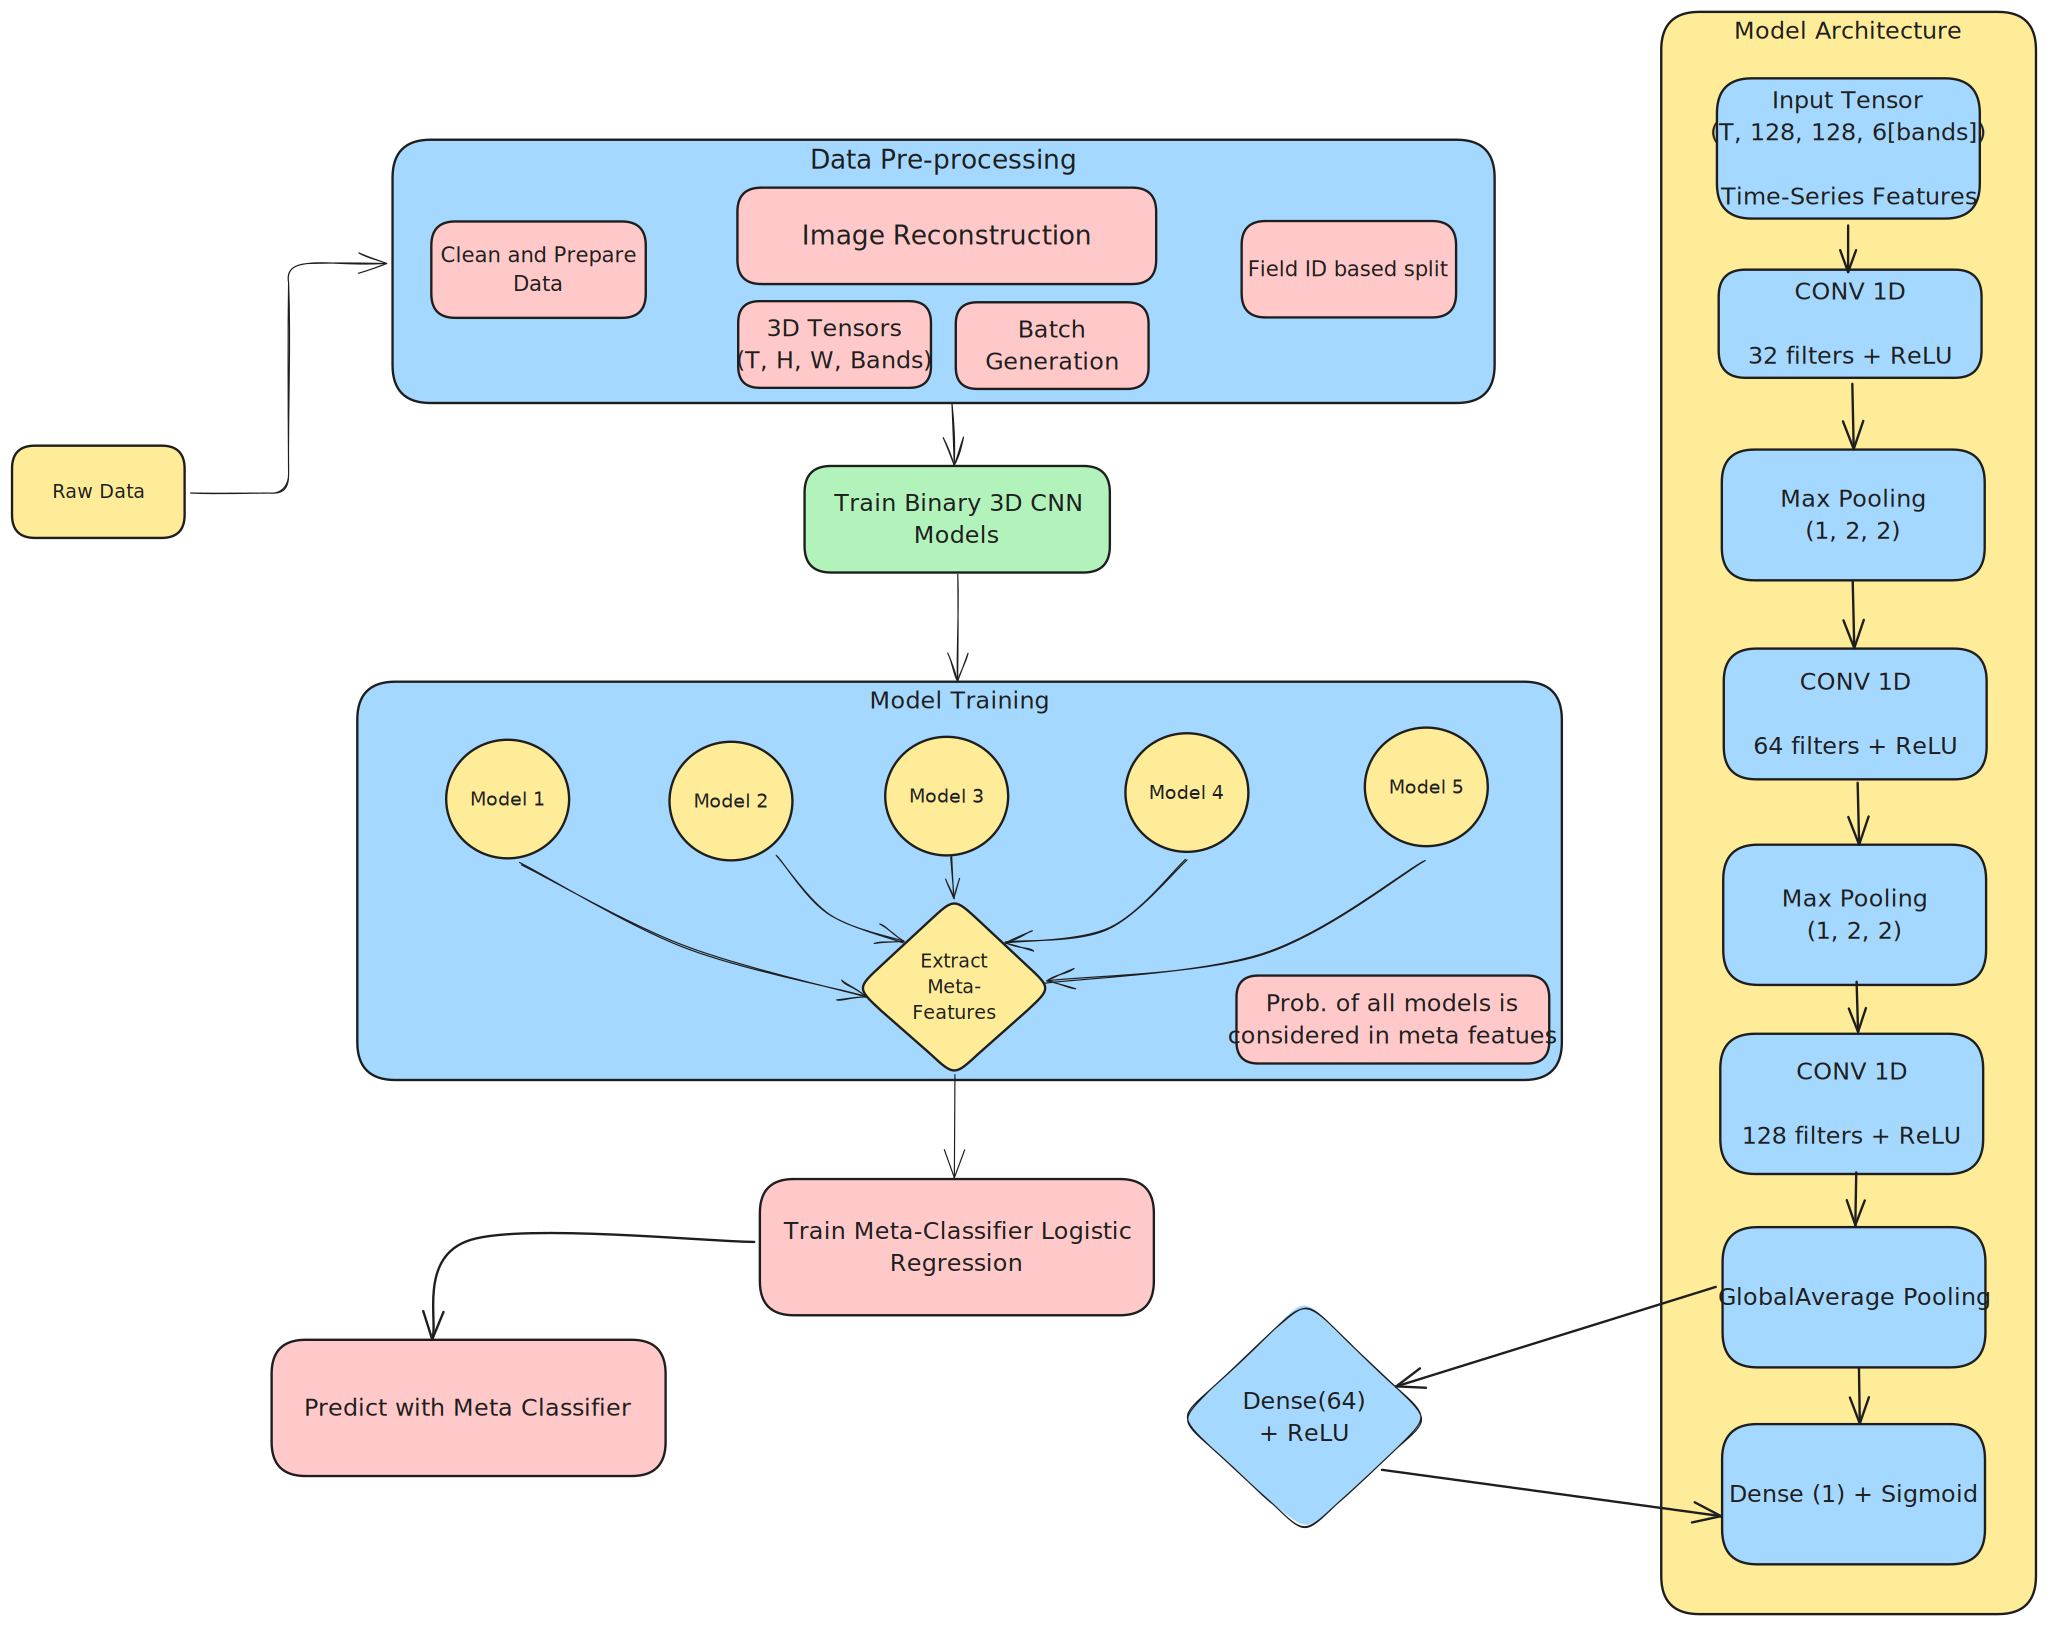
\includegraphics[width=\linewidth]{patch_model.pdf}
        \caption{3D CNN Ensemble Architecture}
        \label{fig:patch_extraction}
        \end{figure}
    
        \item \textbf{Transformer-Based Model:} \\

        In this approach, each patch was flattened into $N=T\times H\times W$ tokens $\{\mathbf{x}_n\}\subset\mathbb{R}^B$ and embedded to $\mathbf{E}\in\mathbb{R}^{N\times d}$. Each multi-head attention layer computes:
        \[
        \begin{aligned}
        \mathrm{Attention}(Q, K, V)
        &= \mathrm{softmax}\left( \frac{QK^\top}{\sqrt{d_k}} \right) V, \\
        Q &= \mathbf{E}W_Q,\quad
        K = \mathbf{E}W_K,\quad
        \\
        V = \mathbf{E}W_V.
        \end{aligned}
        \]
        A final `[CLS]` embedding $\mathbf{h}_\text{CLS}$ is classified by:
        \begin{equation*}
          \hat{\mathbf{p}}
          = \mathrm{softmax}\left(W_\mathrm{cls}\,\mathbf{h}_\text{CLS} + b_\mathrm{cls}\right).
        \end{equation*}
        
        Transformer-based architectures have shown promise in remote sensing by capturing long-range dependencies and global context \cite{ieee2017,cropformer2023}. \\

        \item \textbf{Ensemble of Class-Specific 3D CNNs:} \\

        This ensemble approach combined the outputs of five class-specific 3D CNN experts $f_i(\mathbf{X})=p_i$, each outputting a class probability $p_i$. A logistic regression meta-classifier then combines them:
        \begin{equation*}
          \hat{\mathbf{p}}
          = \mathrm{softmax}\left(W_\mathrm{meta}[p_1,\dots,p_5]^\top + b_\mathrm{meta}\right).
        \end{equation*}
        
        This strategy as depicted by Figure \ref{fig:patch_extraction}, leverages the strengths of specialist models while retaining the robustness of ensemble learning, resulting in the highest performance among patch-level approaches.
        \end{enumerate}
\end{enumerate}

\section{Results and Discussion}

This section presents the main findings of our study, highlighting key performance metrics for each modeling approach. All models were evaluated on an independent, held-out test set to ensure their ability to generalize to unseen data.  

\medskip

\noindent
To account for the highly imbalanced class distribution in our data, we report three metrics that are more informative than overall accuracy:  
\begin{itemize}
  \item \textbf{Cohen’s Kappa (Kappa)}  
    Measures agreement between predicted and true labels, corrected for chance:
    \[
    \kappa = \frac{p_o - p_e}{1 - p_e}, \quad
    p_o = \frac{\text{number of correct predictions}}{N},
    \]
    \[
    p_e = \sum_{c=1}^C \left( \frac{n_{c,\text{true}}}{N} \times \frac{n_{c,\text{pred}}}{N} \right).
    \]
    
  \item \textbf{Weighted F1 Score (F1)}  
    The harmonic mean of precision and recall, weighted by the support of each class:  
    \[
      \mathrm{F1}_{\mathrm{weighted}}
      = \sum_{c=1}^C \frac{n_c}{N}
        \cdot
        \frac{2 \,\text{Precision}_c\,\text{Recall}_c}{\text{Precision}_c + \text{Recall}_c},
    \]
    where \(n_c\) is the number of true instances of class \(c\).
  \item \textbf{Entropy (Log Loss)}  
    Quantifies the average surprise of the predicted probabilities (adapted from the standard cross‐entropy formula):  
    \[
      \mathrm{Entropy}
      = -\frac{1}{N}\sum_{i=1}^N \sum_{c=1}^{5}
         y_{i,c}\,\ln\bigl(p_{i,c}\bigr),
    \]
    where \(y_{i,c}\in\{0,1\}\) is the one‐hot true label for sample \(i\) in class \(c\), \(p_{i,c}\) is the model’s predicted probability for that class, and there are \(5\) crop categories.
\end{itemize}

\noindent
We avoid reporting plain accuracy here because an imbalanced test set can yield deceptively high accuracy simply by predicting the majority class.  In contrast, Cohen’s Kappa and the weighted F1 score reward correct classification across all classes and higher values indicate better agreement and balanced precision/recall, while entropy (log loss) measures prediction uncertainty, so lower values indicate more confident, accurate probability estimates.  


\subsection{Classical Machine Learning}

\subsubsection{Pixel‑Level Analysis}
Table~\ref{tab:cl_ml_pixel_results} summarizes the out-of-sample performance of classical machine learning models at the pixel level. Random Forest achieves the highest performance, with a Cohen’s Kappa of 0.69 and an F1 score of 0.77, indicating substantial agreement beyond chance. Figure~\ref{fig:conf_rf_pixel} shows the confusion matrix of the random forest model at the pixel level.



\begin{table}[htbp]
\centering
\caption{Out-of-sample performance for classical ML pixel-level analysis}
\label{tab:cl_ml_pixel_results}
\renewcommand{\arraystretch}{1.1}
\setlength{\tabcolsep}{6pt}
\begin{tabular}{lccc}
\toprule
\textbf{Model} & \textbf{Kappa} & \textbf{F1} & \textbf{Entropy} \\
\midrule
XGBoost             & 0.68 & 0.76 & 8.47 \\
LightGBM            & 0.66 & 0.74 & 8.90 \\
Random Forest\textsuperscript{\dag} & 0.69 & 0.77 & 7.99 \\
Logistic Regression & 0.65 & 0.73 & 9.07 \\
Voting Classifier   & 0.63 & 0.72 & 9.47 \\
\bottomrule
\end{tabular}
\end{table}
\\

\subsubsection{Field‑Level Analysis}

Table~\ref{tab:ml_field_pixel_results} presents the field-level results for the classical models and ensemble approaches. The Voting Classifier achieves the best performance, with a Cohen’s Kappa of 0.69 and an F1 score of 0.76, highlighting the advantage of ensemble methods over individual classifiers.


\begin{table}[htbp]
\centering
\caption{Out-of-sample performance across classical ML models at pixel and field levels}
\label{tab:ml_field_pixel_results}
\renewcommand{\arraystretch}{1.1}
\setlength{\tabcolsep}{6pt}
\begin{tabular}{lccc}
\toprule
\textbf{Model} & \textbf{Kappa} & \textbf{F1} & \textbf{Entropy} \\
\midrule
XGBoost             & 0.65 & 0.74 & 8.95 \\
LightGBM            & 0.67 & 0.76 & 8.29 \\
Random Forest       & 0.67 & 0.76 & 8.25 \\
Logistic Regression & 0.64 & 0.74 & 9.03 \\
Voting Classifier\textsuperscript{\dag}   & 0.69 & 0.76 & 7.86 \\
Stacking Classifier & 0.67 & 0.75 & 8.55 \\
\bottomrule
\end{tabular}
\end{table}

Combining model predictions at the field level leads to improvements in classification reliability.

Figures~\ref{fig:conf_field_stacking} and~\ref{fig:conf_field_voting} present the confusion matrices for the Stacking and Voting ensemble classifiers evaluated at the field level. Both models demonstrated strong diagonal dominance, indicating high agreement between the predicted and true crop classes.\\

\begin{figure}[ht]
  \centering
  \includegraphics[width=0.85\linewidth]{confusion_matrix_rf_pixel.pdf}
  \caption{Random Forest(Pixel Level) Confusion Matrix}
  \label{fig:conf_rf_pixel}
\end{figure}

For the Stacking Ensemble (Figure~\ref{fig:conf_field_stacking}), lucerne/medics achieves the highest classification accuracy, with over 94\% of fields correctly identified. wheat and canola, however, exhibit some misclassification, particularly as lucerne/medics and barley, which suggests that these classes share spectral-temporal similarities during certain months. The model performs poorly on small grain grazing, with notable confusion spread across barley and wheat, indicating challenges in distinguishing these crops based solely on their seasonal satellite signatures.

In the case of the Voting Ensemble (Figure~\ref{fig:conf_field_voting}), the Cohen's Kappa and F1 score improves, with lucerne/medics again achieving the best performance at over 97\%. The crop wheat is classified more accurately than in the stacking approach, indicating enhanced stability resulting from ensemble consensus. Although minor crops such as barley and small grain grazing continue to show moderate confusion, their misclassification rates are notably lower compared to the stacking strategy, highlighting the robustness of the voting-based aggregation.

These confusion matrices highlight that both ensemble methods effectively consolidate pixel-level predictions into robust field-level outputs. The Voting Ensemble offered better generalization, particularly for dominant crops, while the Stacking Ensemble provides competitive performance across all classes.

\begin{figure}[H]
  \centering
  \includegraphics[width=0.95\linewidth]{confusion_matrix_Stacking Classifier.pdf}
  \caption{Confusion matrix for Stacking Ensemble at field level.}
  \label{fig:conf_field_stacking}
\end{figure}


\begin{figure}[H]
  \centering
  \includegraphics[width=0.95\linewidth]{confusion_matrix_Voting Classifier.pdf}
  \caption{Confusion matrix for Voting Ensemble at field level.}
  \label{fig:conf_field_voting}
\end{figure}
\FloatBarrier

\subsection{Deep Learning}

\subsubsection{Pixel‑Level Analysis}

We evaluated the three models, CNN + BiLSTM + Focal Loss, Ensemble TabTransformer, and 1D CNN with Optuna on a held-out test set.
\begin{itemize}
    
    \item \textbf{Performance Comparison:}

    Table~\ref{tab:final_results} highlight the benefits of temporal modeling and imbalance-aware training for crop classification. The CNN+BiLSTM+Focal Loss model[\ref{fig:conf_matrix_bilstm}] achieved the highest field-level performance, with a Cohen’s Kappa of 0.77 and an F1 score of 0.84, demonstrating superior ability to capture vegetation dynamics and handle class imbalance.
        
    \begin{table}[htbp]
    \centering
    \caption{Comparison of test-set performance across deep learning models at both pixel and field level}
    \label{tab:final_results}
    \renewcommand{\arraystretch}{1.1}
    \setlength{\tabcolsep}{6pt}
    \begin{tabular}{lccc}
    \toprule
    \textbf{Model} & \textbf{Kappa} & \textbf{F1} & \textbf{Entropy} \\
    \midrule
    1D CNN + Optuna            & 0.69 & 0.78 & 8.03 \\
    Ensemble Tab Transformer   & 0.73 & 0.80 & 6.95 \\
    CNN + Bi-LSTM + Focal Loss\textsuperscript{\dag} & 0.77 & 0.84 & 5.91 \\
    \bottomrule
    \end{tabular}
    \end{table}

        The Ensemble TabTransformer achieved a field-level Cohen’s Kappa of 0.73 and an F1 score of 0.80, highlighting the strength of attentive feature selection in high-dimensional crop data~\cite{tabnet2024}. Despite lacking explicit temporal modeling, its sequential decision process effectively captured latent phenological patterns. 
        The 1D CNN, while simpler, still delivered competitive results with a Cohen’s Kappa of 0.69 and an F1 score of 0.78, benefiting from Optuna-based hyperparameter optimization[\ref{tab:optuna_top_trials}]. This supports prior observations~\cite{cnn_optuna} that shallow Conv1D architectures, when carefully tuned, can perform strongly for vegetation classification.

            \begin{figure}[htbp]
            \centering
            \includegraphics[width=0.45\textwidth]{confusion_matrix_bilstm_percent.pdf}
            \caption{Field-level confusion matrix for CNN + BiLSTM ensemble model showing predicted vs. actual crop classes.}
            \label{fig:conf_matrix_bilstm}
            \end{figure}
            
\end{itemize}
\\

\subsubsection{Patch‑Level Analysis}
We evaluated four patch-based deep learning models on spatially coherent image regions extracted from Sentinel-2 tiles. The classification was performed using aggregated patch-level information rather than individual pixels, preserving spatial context and allowing models to exploit neighboring structures. 



\begin{itemize}

    \item \textbf{Performance Comparison:}

        The results suggest that modeling local spatial coherence through patch-level inputs can improve crop classification performance, particularly when ensemble learning strategies are employed. As shown in Table~\ref{tab:dl_patch_results}, the Ensemble Architecture achieved the highest patch-level performance, with a Cohen’s Kappa of 0.66 and an F1 score of 0.75. This ensemble combined outputs from multiple base learners, including CNNs and transformer components, allowing a more generalized understanding of crop field characteristics Figure~\ref{fig:conf_dl_patch}.\\

        Among the individual models as seen in Table~\ref{tab:dl_patch_results}, the 3D CNN performed strongly with a Cohen’s Kappa of 0.65 and an F1 score of 0.74. By capturing volumetric relationships across spectral bands and spatial dimensions, the 3D CNN demonstrated an advantage over traditional 2D methods. The Multi-Channel CNN also achieved competitive results, reaching a Kappa of 0.62 and an F1 score of 0.70. These results highlight the effectiveness of band-specific spatial convolution for capturing vegetation structure and field texture.

        \begin{table}[htbp]
        \centering
        \caption{Out-of-sample performance for deep learning patch-level analysis}
        \label{tab:dl_patch_results}
        \renewcommand{\arraystretch}{1.1}
        \setlength{\tabcolsep}{6pt}
        \begin{tabular}{lccc}
        \toprule
        \textbf{Model} & \textbf{Kappa} & \textbf{F1} & \textbf{Entropy} \\
        \midrule
        Multi-Channel CNN       & 0.62 & 0.70 & 10.57 \\
        3D CNN                  & 0.65 & 0.74 & 8.99 \\
        Transformer-based model & 0.48 & 0.60 & 13.11 \\
        Ensemble Architecture\textsuperscript{\dag} & 0.66 & 0.75 & 8.82 \\
        \bottomrule
        \end{tabular}
        \end{table}
        
        \begin{figure}[H]
          \centering
          \includegraphics[width=0.95\linewidth]{confusion_matrix_3dcnn.pdf}
          \caption{Confusion matrix for 3D CNN Model}
          \label{fig:conf_dl_patch}
        \end{figure}
        

        In contrast, the Transformer-Based Model underperformed, achieving a Cohen’s Kappa of 0.48 and an F1 score of 0.60. This suggests that pure attention-based architectures, without strong inductive biases like spatial locality, may struggle with small patch classification unless extensively pretrained or domain-adapted to remote sensing imagery.
        

\end{itemize}



\section{Discussion}

Our experiments demonstrated that both classical and deep learning approaches can effectively leverage Sentinel-2 imagery for field-level crop classification, yet each paradigm has distinct strengths and limitations. Deep models, particularly the CNN + BiLSTM ensemble trained with Focal Loss, excel at capturing seasonal dynamics and mitigating class imbalance, achieving a 0.77 Cohen's Kappa score at the field level and an F1 score of 0.84. However, they require extensive hyperparameter tuning and  remain sensitive to mixed pixels along field edges due to Sentinel-2’s 10–20 m resolution.

Classical machine learning approaches remained highly competitive: a pixel‐level Random Forest trained on \texttt{xr\_fresh} generated time‐series features generalizes well to unseen data, and a field‐level voting classifier that aggregates those pixel predictions outperforms several deep learning architectures on the held-out test set. By combining SMOTETomek resampling with ensemble methods (like Random Forest, LightGBM, XGBoost) and automated temporal feature engineering, these models achieve comparable or better accuracy with substantially lower computational cost and greater interpretability. However, because they rely primarily on temporal summaries, they do not utilize fine‐scale spatial textures unless supplemented with explicit textural indices.



Our patch-level analysis incorporated spatial context while matching the performance of classical models based on time series features. Dividing each field into fixed-size patches enables 3D CNNs and patch-based ensembles to learn local texture and neighborhood patterns, boost the patch-level Cohen’s Kappa to 0.66. This strategy also provided implicit data augmentation by generating multiple overlapping patches per field, which increases sample diversity and reduces overfitting. However, because patches are placed on a fixed grid, some pixels along field boundaries were left out. Additionally, processing dozens of patches per field significantly increased computational cost and memory requirements.


Looking ahead, several avenues could further improve performance across paradigms:
\begin{itemize}
  \item \textbf{Higher resolution or increased revisit frequency.} PlanetScope or UAV imagery and biweekly acquisitions would reduce edge effects and better capture rapid phenological events. Using all Sentinel 2 observations rather than monthly composites could also achieve the same result.
  \item \textbf{Advanced augmentation.} Spectral band mixing, elastic deformations, or GAN-based patch generation could bolster deep model robustness, particularly for underrepresented crops.
  \item \textbf{Dynamic field delineation and ancillary data.} Change-detection algorithms, soil or elevation maps, and in-situ surveys would strengthen robustness in heterogeneous landscapes.
  \item \textbf{Hybrid workflows.} Combining time-series features with patch-based representation learning may yield a best-of-both-worlds solution—balancing interpretability, spatial detail, and temporal dynamics.
\end{itemize}



\section{Conclusion}

This study presents a comprehensive evaluation of crop classification methods using multi-temporal Sentinel-2 imagery, highlighting the comparative strengths of deep learning, classical machine learning, and patch-based approaches. Our CNN-BiLSTM ensemble, trained with Focal Loss, achieved state-of-the-art performance with an F1 score of 0.84 and a Cohen’s Kappa of 0.77 at the field level, demonstrating the effectiveness of sequence modeling in capturing crop phenological patterns over time. Patch-based methods, particularly the 3D CNN ensemble, contributed valuable spatial context through implicit data augmentation and local texture learning, though at the cost of increased computational demand and the exclusion of edge pixels.

Importantly, we showed that classical machine learning models like LightGBM and XGBoost, when paired with temporal feature extraction via \texttt{xr\_fresh} and class-balancing techniques such as SMOTETomek, offered competitive performance with significantly lower complexity and greater interpretability. These results underscore that classical approaches remain viable and even preferable in resource-constrained or operational settings where model transparency and rapid deployment are essential.

Although this study used a fixed set of 60 hand-crafted temporal and spectral features to capture the dynamics of crop growth, it does not explicitly address the potential issue of redundancy of characteristics or high-dimensional sparsity. We recognize that including many features without a formal selection process may introduce correlated or weakly informative variables, which could affect model generalization or inflate training complexity. Nevertheless, our goal in this work was to establish a comprehensive baseline and evaluate the classification potential of both deep learning and classical models on a rich feature set. Future research should consider incorporating feature optimization and dimensionality reduction strategies to identify the most discriminative features and further enhance model performance.

Looking ahead, future work should focus on multi-source data fusion (e.g., integrating SAR), domain adaptation across regions and growing seasons, and attention-based temporal models to better capture crop-specific phenological traits. Additionally, hybrid workflows that combine temporal feature engineering, spatial representation learning, and scalable inference across high-resolution platforms like PlanetScope hold strong potential to operationalize crop monitoring systems at national and global scales.
  

\bibliographystyle{spmpsci}
\begin{thebibliography}{99}

\bibitem{mdpi2023}
Yunxiang Zhang, Yuxin Zhang, Jun Zhang, Fulin Wang, and Xinyu Wang. (2023). {A Spatio-Temporal Feature Fusion Network for Crop Classification Using Multi-Temporal Sentinel-2 Data}. \textit{ISPRS International Journal of Geo-Information}, 12(11), 450.\href{https://www.mdpi.com/2220-9964/12/11/450}{[Article]}

\bibitem{sciencedirect2023}
S. Ali, M. Usama, M. Usman, M. Rizwan, and A. Rehman, ``A hybrid deep learning model for crop classification using Sentinel-2 time series data,'' \textit{Comput. Electron. Agric.}, vol. 206, p. 107673, 2023. [Online]. Available: \href{https://www.sciencedirect.com/science/article/pii/S0168169923000303}{[Article]}

\bibitem{ieee2017}
A. Ienco, R. Gaetano, C. Dupaquier, and D. H. T. Minh, ``Land cover classification via multitemporal spatial data by deep recurrent neural networks,'' \textit{IEEE Trans. Geosci. Remote Sens.}, vol. 55, no. 4, pp. 2142--2154, 2017. [Online]. Available: \href{https://ieeexplore.ieee.org/document/7891032}{[Article]}

\bibitem{arxiv2024}
Y. Li, Y. Zhang, and Z. Wei, ``Multi-Temporal Crop Classification via Transformer-Based Deep Learning Model,'' arXiv preprint arXiv:2402.02121, 2024. [Online]. Available: \href{https://arxiv.org/abs/2402.02121}{[Article]}

\bibitem{mlhub}
Radiant Earth Foundation, ``South Africa Crop Type Competition,'' Source Cooperative repository, 2024. [Online]. Available: \href{https://github.com/AI4EO/tum-planet-radearth-ai4food-challenge}{[Dataset]}

\bibitem{capstone_repo}
\emph{Capstone\_Group\_3: Source code for multitemporal crop classification},
GitHub repository, 2025.
[Online]. Available: 
\href{https://github.com/DishaKacha7/Capstone_Group_3}{[Github]}


\bibitem{sar2022}
F. Kordi and H. Yousefi, ``Crop classification based on phenology information by using time series of optical and synthetic‐aperture radar images,'' \emph{Remote Sensing Applications: Society and Environment}, vol.~27, art. no. 100812, Jul. 2022. [Online]. Available: \href{https://doi.org/10.1016/j.rsase.2022.100812}{[Article]}


\bibitem{sciencedirect2021}
R. Wang, Y. Wang, Z. Shao, and Y. Zhang, ``Deep learning for crop classification in remote sensing images: A review,'' \textit{ISPRS J. Photogramm. Remote Sens.}, vol. 186, pp. 63--77, 2021. [Online]. Available: \href{https://www.sciencedirect.com/science/article/pii/S0924271623000679}{[Article]}

\bibitem{mann2023}
Michael L. Mann, Lisa Colson, Rory Nealon, Ryan Engstrom, and Stellamaris Nakacwa. (2023). {Lite Learning: Efficient Crop Classification in Tanzania Using Traditional Machine Learning \& Crowd Sourcing}. SSRN Preprint. \href{https://ssrn.com/abstract=5090897}{[Article]}


\bibitem{medium2023}
A. Chauhan, ``Crop Classification via Satellite Image Time Series and PSETAE Deep Learning Model,'' Medium, 2023. [Online]. Available: \href{https://medium.com/geoai/crop-classification-via-satellite-image-time-series-and-psetae-deep-learning-model-c685bfb52ce}{[Article]}

\bibitem{kuwait2023}
A. K. Rangarajan, R. Purushothaman, M. Prabhakar, and C. Szczepański, ``Crop identification and disease classification using traditional machine learning and deep learning approaches,'' \textit{J. Eng. Res.}, vol. 11, no. 1B, pp. 1--12, 2023. [Online]. Available: \href{https://kuwaitjournals.org/jer/index.php/JER/article/view/11941}{[Article]}

\bibitem{acm2020}
K. K. Gadiraju, B. Ramachandra, Z. Chen, and R. R. Vatsavai, ``Weakly supervised deep learning for rapid crop cover mapping with multi-temporal satellite imagery,'' in \textit{Proc. 26th ACM SIGKDD Int. Conf. Knowl. Discov. Data Min.}, 2020. [Online]. Available: \href{https://dl.acm.org/doi/abs/10.1145/3394486.3403375}{[Article]}

\bibitem{liu2022}
X. Liu et al., ``Deep learning for crop classification,'' \textit{IEEE Transactions on Geoscience and Remote Sensing}, vol. 60, pp. 1-14, 2022. [Online]. Available: \href{https://example.com/liu2022}{[Article]} % Replace with actual URL

\bibitem{zhang2023}
Y. Zhang et al., ``Transformer-based crop classification,'' \textit{ISPRS Journal of Photogrammetry}, vol. 195, pp. 200-215, 2023. [Online]. Available: \href{https://example.com/zhang2023}{[Article]} % Replace with actual URL

\bibitem{nasa2023}
NASA/IBM, ``Prithvi-100M technical report,'' Tech. Rep., 2023. [Online]. Available: \href{https://example.com/prithvi}{[Report]} % Replace with actual URL

\bibitem{khan2024}
Z. Khan et al., ``Ensemble methods for precision agriculture,'' \textit{Computers and Electronics in Agriculture}, vol. 216, p. 108495, 2024. [Online]. Available: \href{https://example.com/khan2024}{[Article]} % Replace with actual URL

\bibitem{wang2022}
L. Wang et al., ``Multi-temporal crop classification,'' \textit{Agricultural Systems}, vol. 203, p. 103517, 2022. [Online]. Available: \href{https://example.com/wang2022}{[Article]} % Replace with actual URL

\bibitem{russwurm2018}
M. Rußwurm and M. Körner, ``Temporal CNN for crop analysis,'' \textit{Remote Sensing}, vol. 10, no. 12, p. 1930, 2018. [Online]. Available: \href{https://example.com/russwurm2018}{[Article]} % Replace with actual URL

\bibitem{sa_comp}
Radiant Earth Spot The Crop Challenge \href{https://github.com/radiantearth/spot-the-crop-challenge}{[Github]} % Replace with actual URL



\bibitem{campbell2011introduction}
James B. Campbell and Randolph H. Wynne. (2011). \textit{Introduction to Remote Sensing}. The Guilford Press.

\bibitem{mann2024xr_fresh}
Michael L. Mann. (2024). \textit{mmann1123/xr\_fresh: SpeedySeries (0.2.0)}. Zenodo. \href{https://doi.org/10.5281/zenodo.12701466}{[Software]}


\bibitem{wardlow2007towards}
B. D. Wardlow, S. N. Melendez, and C. M. Justice, ``Towards an operational system for cropland monitoring using MODIS time series data,'' \textit{Remote Sens. Environ.}, vol. 110, no. 3, pp. 349--361, 2007.

\bibitem{james2013}
Gareth James, Daniela Witten, Trevor Hastie, and Robert Tibshirani. (2013). \textit{An Introduction to Statistical Learning}. Springer.

\bibitem{breiman2001}
Leo Breiman. (2001). Random forests. \textit{Machine Learning}, 45(1), 5-32.

\bibitem{biau2008}
Gérard Biau. (2008). Consistency of random forests. \textit{The Annals of Statistics}, 36(4), 2032-2068.

\bibitem{ke2017}
Guolin Ke, Qi Meng, Thomas Finley, Taifeng Wang, Wei Chen, Weidong Ma, Qiwei Ye, and Tie-Yan Liu. (2017). LightGBM: A highly efficient gradient boosting decision tree. \textit{Advances in Neural Information Processing Systems}, 30.

\bibitem{chen2016}
Tianqi Chen and Carlos Guestrin. (2016). XGBoost: A scalable tree boosting system. In \textit{Proceedings of the 22nd ACM SIGKDD International Conference on Knowledge Discovery and Data Mining} (pp. 785-794).

\bibitem{friedman2001}
Jerome H. Friedman. (2001). Greedy function approximation: a gradient boosting machine. \textit{Annals of Statistics}, 29(5), 1189-1232.

\bibitem{dietterich2000}
Thomas G. Dietterich. (2000). An experimental comparison of three methods for constructing ensembles of decision trees: Bagging, boosting, and randomization. \textit{Machine Learning}, 40(2), 139-157.

\bibitem{maxwell2019}
Aaron E. Maxwell, Timothy A. Warner, and Fang Fang. (2019). Implementation of machine-learning classification in remote sensing: an overview. \textit{Remote Sensing}, 11(14), 1633.

\bibitem{zhu2017}
Xiao Xiang Zhu, Devis Tuia, Lorenzo Mou, Gui-Song Xia, Liangpei Zhang, Feng Xu, and Friedrich Fraundorfer. (2017). Deep learning in remote sensing: A comprehensive review and list of resources. \textit{IEEE Geoscience and Remote Sensing Magazine}, 5(4), 8-36.

\bibitem{li2019}
Rui Li, Shuang Zheng, Chao Zhang, and Chenguang Huang. (2019). Object detection in remote sensing images based on improved Faster R-CNN. \textit{IEEE Access}, 7, 35813-35822.

\bibitem{ijabs2020}
I. Ijabs, ``Artificial Intelligence and Democracy: A Political-Theoretical Perspective,'' \textit{Baltic Journal of Modern Computing}, vol. 8, no. 4, pp. 607--616, 2020. [Online]. Available: \href{https://www.bjmc.lu.lv/fileadmin/user_upload/lu_portal/projekti/bjmc/Contents/10_4_02_Ijabs.pdf}{[Article]}

\bibitem{review_dl_crops} 
J. A. et al., ``Deep Learning Models for the Classification of Crops in Aerial Imagery: A Review,'' \textit{Remote Sensing Reviews}, vol. 46, no. 1, pp. 1–24, 2023. [Online]. Available: \href{https://www.sciencedirect.com/science/article/pii/S0168169923000303}{[Article]}

\bibitem{cnn_multitemp} 
N. Kussul, M. Lavreniuk, S. Skakun, and A. Shelestov, ``Deep Learning Classification of Land Cover and Crop Types Using Remote Sensing Data,'' \textit{IEEE Geoscience and Remote Sensing Letters}, vol. 14, no. 5, pp. 778--782, May 2017. doi: 10.1109/LGRS.2017.2681128. [Online]. Available: \href{https://ieeexplore.ieee.org/document/7890411}{[Article]}

\bibitem{tabnet2024} 
A. K. et al., ``A Deep Learning Approach for Dealing with Tabular Data in Crop Classification,'' \textit{IEEE Access}, 2024. [Online]. Available: \href{https://ieeexplore.ieee.org/abstract/document/10826760}{[Article]}

\bibitem{cnn_optuna} 
``Deep learning based multi-temporal crop classification,'' \textit{Remote Sensing of Environment}, vol. 221, pp. 175--190, 2019. [Online]. Available: \href{https://www.sciencedirect.com/science/article/abs/pii/S0034425718305418}{[Article]}

\bibitem{rustowicz2019}
Ryan M. Rustowicz, A. Singh, M., and A. Davis. (2019). Semantic segmentation of crop type in African smallholder agriculture. In \textit{Proceedings of the IEEE/CVF Conference on Computer Vision and Pattern Recognition Workshops} (pp. 75-82).

\bibitem{ji2018}
Shaowu Ji, Chenglong Shen, Yuxiang Zhu, Shuang Zhang, and Yanfeng Lu. (2018). 3D convolutional neural networks for crop classification with multi-temporal remote sensing images. \textit{Remote Sensing}, 10(1), 75.

\bibitem{cropformer2023}
Y. Zhao, W. Li, M. Li, and J. Wang, ``Cropformer: A new generalized deep learning classification framework for multi-scenario crop classification,'' \textit{Front. Plant Sci.}, vol. 14, p. 1130659, 2023. [Online]. Available: \href{https://www.frontiersin.org/articles/10.3389/fpls.2023.1130659/full}{[Article]}

\bibitem{sciencedirect2021b}
M. O. Turkoglu, S. D'Aronco, G. Perich, F. Liebisch, C. Streit, K. Schindler, and J. D. Wegner, ``Crop Type Classification with Satellite Imagery Using Deep Learning,'' \textit{Remote Sens. Environ.}, vol. 256, p. 112331, 2021. [Online]. Available: \href{https://www.sciencedirect.com/science/article/pii/S0034425721003230}{[Article]}

\bibitem{ref_medium} 
``Crop Classification via Satellite Image Time Series and PSETAE Deep Learning Model,'' Medium. [Online]. Available: \href{https://medium.com/geoai/crop-classification-via-satellite-image-time-series-and-psetae-deep-learning-model-c685bfb52ce}{[Article]}

\bibitem{ref_mdpi} 
``Crop Classification with Satellite Data,'' \textit{MDPI Proceedings}, vol. 82, no. 1, p. 95, 2024. [Online]. Available: \href{https://www.mdpi.com/2673-4591/82/1/95}{[Article]}

\bibitem{ref_acm} 
``Crop Monitoring with Deep Learning on Satellite Data,'' in \textit{ACM KDD}, 2020. [Online]. Available: \href{https://dl.acm.org/doi/abs/10.1145/3394486.3403375}{[Article]}

\bibitem{ref_rse2021} 
``Crop Type Classification with Satellite Imagery Using Deep Learning,'' \textit{Remote Sensing of Environment}, 2021. [Online]. Available: \href{https://www.sciencedirect.com/science/article/pii/S0034425721003230}{[Article]}

\bibitem{ref_jer} 
``Crop Classification using Machine Learning and Remote Sensing,'' \textit{Journal of Engineering Research}, 2022. [Online]. Available: \href{https://kuwaitjournals.org/jer/index.php/JER/article/view/11941}{[Article]}

\end{thebibliography}


\end{document}
